\documentclass[10pt,letterpaper]{article}
\usepackage[margin=0.67in,top=0.62in,bottom=0.65in]{geometry}
\usepackage[T1]{fontenc}
\usepackage{mathptmx,amsmath,amssymb,graphicx,booktabs,tabularx,array,xcolor,tikz,enumitem}
\usetikzlibrary{arrows.meta,positioning,calc}
\usepackage[hidelinks]{hyperref}
\usepackage{fancyhdr}
\pagestyle{fancy}\fancyhf{}\renewcommand{\headrulewidth}{0pt}
\fancyfoot[C]{\small\thepage}
\setlength{\headheight}{14pt}
\setlength{\parindent}{0pt}\setlength{\parskip}{4pt}
\setlength{\tabcolsep}{4pt}
\renewcommand{\arraystretch}{1.10}
\newcolumntype{L}[1]{>{\raggedright\arraybackslash}p{#1}}
\newcolumntype{Y}{>{\raggedright\arraybackslash}X}
\newcommand{\heading}[1]{\vspace{5pt}{\large\bfseries #1}\par\vspace{1pt}}
\newcommand{\subhead}[1]{\textbf{#1}\ }
\newcommand{\code}[1]{\texttt{\small #1}}
\definecolor{accent}{RGB}{35,75,105}
\definecolor{pale}{RGB}{239,244,247}
\hypersetup{pdftitle={Robot Joint Digital Twin Data Measurement and Uncertainty},pdfauthor={Zhaoyang Guo, Zhengjie Cui, Junchi Fan}}
\begin{document}
{\small CMU 12-831 Digital Twins and AI for Predictive Analytics \hfill November 15, 2026}\\[4pt]
{\LARGE\bfseries Data and Uncertainty for a Robot Joint Digital Twin}\\[4pt]
{\large Final Project Deliverable 2}\\[3pt]
Zhaoyang Guo \quad Zhengjie Cui \quad Junchi Fan

We characterize the measurement foundation of the joint twin introduced in Deliverable 1 (D1), focusing on axis 2. The immediate objective is reliable friction detection, fault classification and decision replay. Existing recorded-data analyses support this objective; remaining experiments will test sensitivity to measurement error and data splitting. Cycles-to-limit remains an optional simulation study, since the data contain no observed wear-to-failure history.

\heading{2.1 Physical System and Measurement Model}
The six-axis Yu-Cobot performs a pick-and-place task with a vacuum gripper and a can [1]. The archive contains 2122 cycles: 1367 normal and 755 with induced anomalies. Our spatial boundary is the shoulder joint and its downstream load. Figure 1 shows the functional locations of the observed signals. Geometry is schematic; link dimensions and sensor mounting tolerances are not established here.

\begin{center}
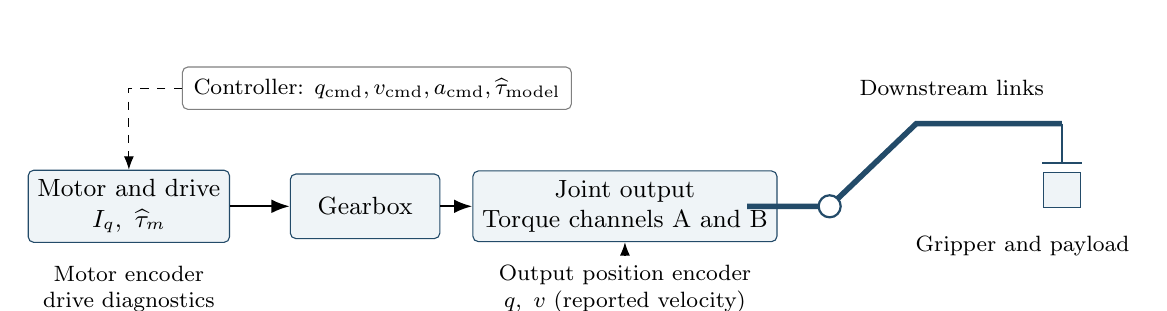
\begin{tikzpicture}[x=1cm,y=1cm,>=Latex,font=\small,
box/.style={draw=accent,rounded corners=2pt,fill=pale,align=center,minimum height=.82cm},
lab/.style={font=\footnotesize,align=center}]
\node[box,minimum width=2.45cm] (motor) at (1.25,0) {Motor and drive\\$I_q,\ \widehat{\tau}_{m}$};
\node[box,minimum width=1.9cm] (gear) at (4.25,0) {Gearbox};
\node[box,minimum width=3.05cm] (out) at (7.55,0) {Joint output\\Torque channels A and B};
\draw[->,thick] (motor)--(gear);
\draw[->,thick] (gear)--(out);
\draw[line width=2pt,accent] (9.1,0)--(10.15,0)--(11.25,1.05)--(13.1,1.05);
\filldraw[fill=white,draw=accent,thick] (10.15,0) circle(.14);
\draw[accent,thick] (13.1,1.05)--(13.1,.55);
\draw[accent,thick] (12.85,.55)--(13.35,.55);
\draw[fill=pale,draw=accent] (12.87,-.02) rectangle (13.33,.43);
\node[lab] at (11.7,1.5) {Downstream links};
\node[lab] at (12.6,-.5) {Gripper and payload};
\node[lab] (enc) at (7.55,-1.05) {Output position encoder\\$q,\ v$ (reported velocity)};
\draw[->] (enc.north)--(out.south);
\node[lab] at (1.25,-1.05) {Motor encoder\\drive diagnostics};
\node[lab,draw=gray,rounded corners=2pt,inner sep=4pt] (ctrl) at (4.4,1.5)
{Controller: $q_{\rm cmd},v_{\rm cmd},a_{\rm cmd},\widehat{\tau}_{\rm model}$};
\draw[->,dashed] (ctrl.west)-|(motor.north);
\end{tikzpicture}\\[-2pt]
{\footnotesize Figure 1. Functional joint and sensing schematic, not a hardware cross-section. Solid arrows show the mechanical chain; the dashed arrow denotes commands. A/B are treated as two reported torque channels.}
\end{center}

Gravity, inertia, friction and external load determine joint torque. A useful measurement description is
\[
y_A(t)=\tau_{\rm out}(t)+\beta_A(t)+\eta_A(t)+e_{Q,A}(t),
\qquad
r(t)=y_A(t)-\widehat{\tau}_{\rm model}(t),
\]
where $\beta_A$, $\eta_A$ and $e_{Q,A}$ denote bias, random variation and quantization. The controller torque is a model estimate, not an independent reference measurement. In each cycle the implemented least-squares fit is
\[
r(t)=c_0+\tau_c\,\operatorname{sign}(v(t))+b\,v(t)+\Delta J\,a_{\rm cmd}(t)+\epsilon(t).
\tag{1}
\]
Here $q$ is in rad, $v$ in rad/s, $a_{\rm cmd}$ in rad/s$^2$, $c_0$ and $\tau_c$ in N\,m, $b$ in N\,m\,s/rad and $\Delta J$ in kg\,m$^2$ (radians dimensionless). \textbf{The code uses commanded acceleration as a proxy for actual acceleration}; tracking error is part of model uncertainty. The coefficient $\tau_c$ is an effective friction-related indicator, not an identified physical friction torque. Bias, imperfect gravity compensation, trajectory changes and omitted dynamics can enter the fitted coefficients and residual.

\subhead{Scales and existing evidence.}
The nominal interval is 10 ms; one cycle averages 11.01 s, and the twin updates once per completed cycle. Healthy axis-2 positions span 1.197--1.584 rad in the analyzed data. Existing fits [3] give healthy $\tau_c=0.579\pm0.172$ N\,m ($n=1367$, mean $\pm$ cycle SD), versus $1.834\pm0.242$ ($n=11$, A2\_B) and $3.033\pm0.350$ ($n=10$, A2\_A). These are recorded, artificially induced friction conditions, not stages of observed aging.

\heading{2.2 Sensing Sampling and Data Acquisition}
The source authors report RLS AksIM-2 position encoders, Sensodrive GMS torque sensing, EtherCAT communication between axes and controller, and network capture with \emph{tshark} at 500 Hz [1]. We use the public 100 Hz Parquet release [2]. Joint torque and position channels are measurements; motor torque and controller torque are estimates. Drive-reported current components are not independent torque standards.

\newpage
\heading{2.2 Sensing Sampling and Data Acquisition Continued}
\begin{center}
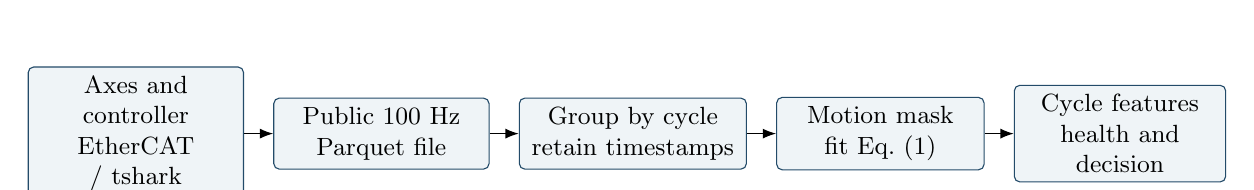
\begin{tikzpicture}[>=Latex,font=\small,node distance=.37cm,
box/.style={draw=accent,fill=pale,rounded corners=2pt,align=center,minimum height=.85cm}]
\node[box,text width=2.5cm] (a) {Axes and controller\\EtherCAT / tshark};
\node[box,text width=2.5cm,right=of a] (b) {Public 100 Hz\\Parquet file};
\node[box,text width=2.65cm,right=of b] (c) {Group by cycle\\retain timestamps};
\node[box,text width=2.4cm,right=of c] (d) {Motion mask\\fit Eq.\ (1)};
\node[box,text width=2.45cm,right=of d] (e) {Cycle features\\health and decision};
\draw[->] (a)--(b);\draw[->] (b)--(c);\draw[->] (c)--(d);\draw[->] (d)--(e);
\end{tikzpicture}\\[2pt]
{\footnotesize Figure 2. Acquisition and local analysis path. The archive supplies aligned rows; physical channel timing accuracy is unverified. Labels are retained for grouping and evaluation, not used as predictor features.}
\end{center}

\subhead{Sampling and resolution.}
Within-cycle timestamps have median spacing 10.067 ms (about 99.3 Hz), averaging 1094 samples per cycle. No spacing exceeded $1.5$ times the median; this checks gaps, not all missing values or synchronization. At nominal 100 Hz, the mean Welch spectrum of the first 300 healthy cycles places 99\% of axis-2 torque-A power below 8.594 Hz. This supports cycle-level friction monitoring but cannot rule out prior aliasing. Hardware bit depths, channel skew and filtering used for the 100 Hz release remain unverified.

Observed increments are about 0.011 N\,m for torque A/B and $5.96\times10^{-6}$ rad for position: empirical logged-value spacings, not hardware specifications. The torque increment is small relative to the 0.165 N\,m stationary fluctuation. Compare matched 500 Hz cycles with explicitly low-pass-filtered 100 Hz data in a follow-up check.

\subhead{Preprocessing actually implemented.}
Group axis records by \code{sample}, preserving within-cycle row order and time. Fit on $|v|>0.02$ rad/s with at least 20 moving samples, without additional filtering, differentiation or resampling. For noise, demean stationary segments of at least 30 samples with $|v|<0.005$ rad/s and $v_{\rm cmd}=0$. Classifier scaling is fitted in training pipelines; physical fits retain engineering units. Add timestamp, finite-value and rank checks before fitting; reject unusable cycles rather than interpolate across gaps.

\heading{2.3 Variable and Uncertainty Budget}
Table 1 lists core fit and diagnostic streams. \textbf{Every input row: nominal 100 Hz; data provenance/owner: voraus-AD providers} (voraus robotik and research collaborators [1,2]); license CC BY-NC-SA 4.0. Our team derives $\tau_c$ once per cycle.

{\small
\begin{tabularx}{\linewidth}{@{}L{2.45cm}L{2.7cm}L{1.55cm}L{1.65cm}Y@{}}
\toprule
\textbf{Stream / meaning} & \textbf{Source} & \textbf{Unit} & \textbf{Rest SD} & \textbf{Main bias / limitation}\\
\midrule
$q$: joint angle & Output encoder & rad & $9.76\,10^{-5}$ & Calibration; tracking error\\
$v$: joint speed & Reported velocity & rad/s & 0.00195 & Filter delay; near-zero sign\\
$y_A$: output torque & Torque channel A & N\,m & 0.165 & A--B mean: $+0.741$ N\,m\\
$y_B$: output torque & Torque channel B & N\,m & 0.162 & Shared errors with A\\
$I_q$: motor current & Drive component & A & 0.0569 & Current scale; thermal effects\\
$\widehat{\tau}_m$: motor torque & Drive estimate & N\,m & 0.798 & Torque constant; transmission\\
$\widehat{\tau}_{\rm model}$: torque & Controller model & N\,m & N/A & A--model mean: $-7.21$ N\,m\\
$q_{\rm cmd},v_{\rm cmd},a_{\rm cmd}$ & Controller commands & rad, rad/s, rad/s$^2$ & N/A & Command--state mismatch\\
$I_{\rm robot}$: supply current & Whole-arm channel & A & 0.184 & Not axis-local; offset\\
$t$: cycle time & Archive timestamp & s & $15.9\,\mu$s$^*$ & Clock accuracy / skew unknown\\
\bottomrule
\end{tabularx}
}
{\footnotesize Table 1. Nominal frequency: 100 Hz for all inputs; common ownership is stated above. Rest SD is $\sqrt{\text{mean stationary-segment variance}}$, not calibrated sensor accuracy. $^*$Time reports interval SD, not signal noise. N/A denotes computed or commanded streams without an assigned sensor-noise estimate. Absolute calibration is unavailable; channel/model differences do not establish absolute bias.}

\heading{2.3 Error Interpretation and Propagation}
\subhead{Random variation and systematic effects.}
Stationary fluctuations can include control action and residual motion as well as electronics noise. A/B disagreement identifies inconsistency, but neither channel establishes the true torque. The stationary A--B mean (0.741 N\,m) and the D1 whole-cycle mean (about 0.47 N\,m) use different motion regimes. Position--command differences likewise include control tracking. Across healthy recording batches, the SD of the mean $\tau_c$ is 0.030 N\,m, versus an average within-batch SD of 0.167 N\,m; batch variability therefore needs monitoring even though it is relatively small for this indicator.

\subhead{Propagation to the health indicator.}
For a fixed design matrix $X=[1,\operatorname{sign}(v),v,a_{\rm cmd}]$, a response perturbation gives
$\delta\widehat{\boldsymbol{\beta}}=(X^\top X)^{-1}X^\top\delta r$.
An additive constant in torque is absorbed by $c_0$ when $X$ has full rank. Direction-dependent errors can shift $\tau_c$; gain errors, velocity errors, timing offsets and imperfect acceleration proxies can affect several coefficients. Correlated residuals limit the benefit of averaging. The observed healthy cycle-to-cycle SD of $\tau_c$ is 0.172 N\,m; the mean within-cycle fit-residual SD is 2.301 N\,m. They describe different statistical levels and neither is the calibrated torque-sensor accuracy.

\subhead{Management and calibration.}
Use training-only healthy bands to monitor A/B mean and spread and cycle duration; flag unreliable cycles and abstain from a fault-specific decision. This does not detect all common-mode errors. Absolute calibration would require a known applied torque/reference transducer and encoder reference, unavailable in this dataset. Preserve offsets for diagnosis rather than forcing channels to agree. Missing values, nonmonotonic/duplicate times and large gaps will be logged and rejected before fitting. Channel-shift tests will bound sensitivity to latency; the present once-per-cycle system does not provide real-time protective stopping.

\heading{Cross-Axis Context and Reproducibility}
\subhead{Six-axis comparison.}
The same fitting and uncertainty routines were applied to all axes [3]. Negative fitted $\tau_c$ values emphasize the need for axis-specific baselines and caution about controller models, sign conventions and parameter identifiability.

\begin{center}
\begin{tabular}{@{}crrrrr@{}}
\toprule
Axis & Healthy $\overline{\tau_c}$ & Healthy SD & Torque-A $\sigma_{\rm rest}$ & Logged increment & Torque-A $f_{99}$\\
 & N\,m & N\,m & N\,m & N\,m & Hz\\
\midrule
1 & 0.150 & 0.0846 & 0.511 & 0.01122 & 10.94\\
\textbf{2} & \textbf{0.579} & \textbf{0.1720} & \textbf{0.165} & \textbf{0.01100} & \textbf{8.59}\\
3 & $-0.597$ & 0.0938 & 0.177 & 0.01095 & 33.98\\
4 & 0.199 & 0.0266 & 0.0762 & 0.00286 & 46.88\\
5 & $-0.0210$ & 0.0174 & 0.0387 & 0.00293 & 45.31\\
6 & 0.119 & 0.00706 & 0.0137 & 0.00276 & 49.22\\
\bottomrule
\end{tabular}
\end{center}
{\small Table 2. Healthy $\tau_c$ statistics use 1367 cycles per axis. Spectra use the first 300 healthy cycles in sorted cycle-ID order, not a random or necessarily chronological sample. $f_{99}$ is the frequency below which 99\% of the averaged, demeaned Welch spectral power lies.}

The strong low-frequency concentration on axis 2 does \emph{not} justify the same sampling conclusion for every joint: axes 4--6 have appreciable power close to the nominal 50 Hz Nyquist limit. A 500 Hz comparison is particularly relevant before extending transient detection to those axes.

\subhead{Estimation limits.}
Logged increments use the smallest positive spacing among the first 400,000 healthy values; floating-point spacing may dominate, so these are not hardware bit depths or ENOB. Stationary segments are demeaned and equally weighted. Conventional and heuristic correlation-adjusted mean standard errors for axis-2 $\tau_c$ are 0.171 and 0.543 N\,m (mean residual lag-one correlation 0.818); neither adjustment nor the simplified quantization-averaging estimate is a validated regression confidence interval. A design-aware covariance or within-cycle block bootstrap remains a follow-up check.

\subhead{Evidence and reproducibility.}
All numerical summaries in this report were transcribed or recomputed from saved result tables at project commit \code{e889be13e25c536dbddf0a0d6340edbf8634f047}. They are not the outcome of a new full run. The raw Parquet file is downloaded separately; without it, scripts 01--05 cannot be fully reproduced. The D2 source is maintained alongside the course documents.

{\footnotesize Evidence files: \code{results/01\_explore/cycles\_axis*.csv}; \code{results/02\_uncertainty/}; fitting and feature definitions in \code{twin/physics.py}, \code{twin/uncertainty.py}, \code{twin/features.py}; detection and replay in \code{twin/detect.py} and \code{scripts/05\_replay.py}.}



\begin{minipage}{\linewidth}
\heading{Preliminary Dashboard Development}
We have begun developing a local dashboard to visualize joint condition and replay saved results without retraining. Figure 3 shows the preliminary interface: the indicator uses a saved recorded-cycle result, while the arm trajectory is schematic. Displayed limits and actions are prototype outputs, not validated operating recommendations.

\begin{center}
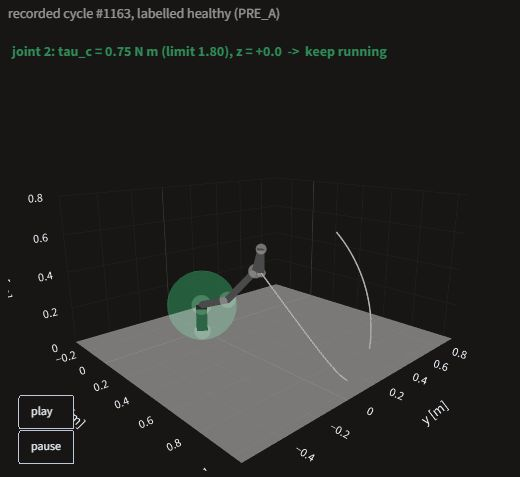
\includegraphics[width=0.36\linewidth]{images/dashboard_prototype.jpg}\\[5pt]
\parbox{0.92\linewidth}{\small\textbf{Figure 3.} Actual preliminary dashboard screenshot (November 15, 2026), cropped to the schematic arm and axis-2 friction indicator for recorded healthy cycle 1163 (PRE\_A). Interface development and validation are ongoing.}
\end{center}

\end{minipage}

\heading{Future Work and Remaining Experiments}
Repeat 70/30 train/test splits with seeds 0--9, keeping complete cycles together and stratifying by class and friction level. Fit preprocessing and thresholds using training data only. Report mean, SD and test counts across seeds, with a separate healthy-batch holdout check. The tests below remain planned work.

{\small
\begin{tabularx}{\linewidth}{@{}L{2.4cm}Y L{4.7cm}@{}}
\toprule
\textbf{Test} & \textbf{Comparison} & \textbf{Main outcome}\\
\midrule
Healthy baseline & Train on healthy cycles; hold out batches. & False alarms, abstention, baseline drift.\\
Friction sensitivity & Test both recorded axis-2 friction levels. & Recall by level; compare with torque RMS.\\
Specificity & Added payload and other-axis friction. & False axis-2 friction calls.\\
Sensor integrity & Add A-only offsets; retain B as recorded. & Abstention and change in $\tau_c$.\\
Timing and noise & Shift torque by 1--2 samples; add noise. & Changes in $\tau_c$ and detection.\\
\bottomrule
\end{tabularx}
}

\subhead{TA feedback and priorities.}
Following the TA's D1 feedback, prioritize fault detection, classification and the decision layer, and repeat complete-cycle train/test splits with several random seeds. Scripts 03 and 05 provide infrastructure; the stability summary and offset sweep above remain to be run. Save seeds, cycle IDs, thresholds and metrics. Cycles-to-limit (script 04) is optional: simulated degradation cannot be validated against real wear with this dataset.

\subhead{Dashboard development.}
Refine the interface and navigation; improve the workflow for launching analyses, inspecting progress and selecting completed runs; make recorded, estimated and simulated quantities explicit throughout the interface; and connect data-quality flags and abstention explanations to the displayed indicators. Validate the integrated workflow and its decision outputs using the complete-cycle, multi-seed protocol in the main text. Live robot connectivity, deployment and operational validation are not demonstrated by this screenshot.


{\small\subhead{Use of generative AI.}
A generative AI assistant was used to help with coding (writing and debugging parts of the analysis scripts) and to polish the text of this report. The problem definition, the modelling choices and the analysis are the team's own.}

\heading{References}
{\small
[1] J. T. Brockmann, M. Rudolph, B. Rosenhahn and B. Wandt. \emph{The voraus-AD Dataset for Anomaly Detection in Robot Applications}. IEEE Transactions on Robotics, 2024. Source methods: Sec.\ III and Table II of the authors' preprint, \url{https://arxiv.org/abs/2311.04765}.

[2] voraus robotik. \emph{voraus-AD dataset and official code repository}. Public 100 Hz and 500 Hz releases; CC BY-NC-SA 4.0 dataset license. \url{https://github.com/vorausrobotik/voraus-ad-dataset}.

[3] Z. Guo, Z. Cui and J. Fan. \emph{Robot joint twin}, code and saved analysis outputs, commit \code{e889be1}. \url{https://github.com/zg2-pixel/robot-joint-twin/tree/e889be13e25c536dbddf0a0d6340edbf8634f047}. D1: \emph{A Predictive Digital Twin of a Robot Joint}, CMU 12-831, November 8, 2026.
}

\end{document}
